\subsection{Brief}
\paragraph{System Requirements}
the proposed system should:
\begin{enumerate}[noitemsep,nolistsep]
	\item correctly detect faces within input images.
	\item provide an accurate model to classify facial expressions.
	\item keep a high performance suitable for real time processing on videos.
\end{enumerate}
\paragraph{our objective} is to build a library that provides the user with an easy to use API that enables him to extracts faces emotions from the given input image, video, or live streaming video, as well as providing lower level API to help the user to build his own facial expression detection model such as image enhancements, face-tracking and face-detection.
\subsection{System blocks}
the System we propose is made of multiple blocks each which is independent of one another yet can interact together to achieve the targeted results, Figure 
\ref{fig:facial_expression_detection} shows the different blocks of our system conceptually and how they interact together in the process of classification of facial expressions, in the next few section we will brief on each those blocks, and what is their task. 

\begin{figure}
	\centering
	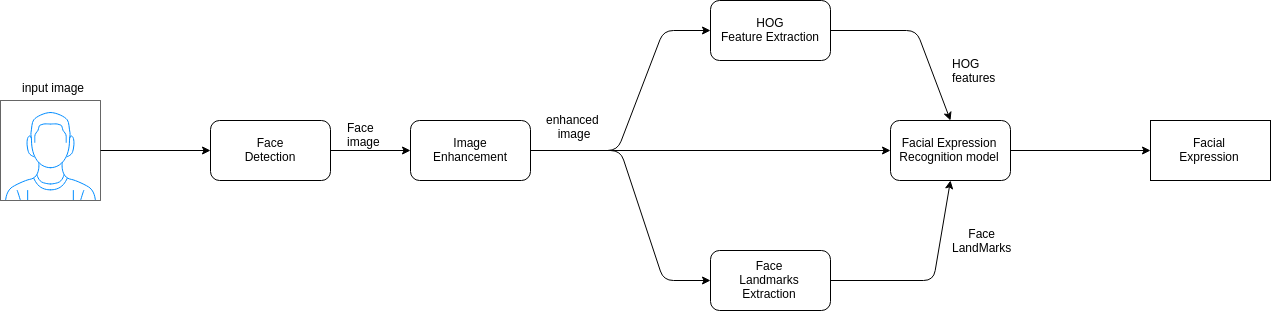
\includegraphics[width=\textwidth]{images/facial_expression_detection.png}
	\caption{Conceptual diagram of different blocks}
	\label{fig:facial_expression_detection}
\end{figure}

\paragraph{face detection}
since our job with the model is to classify the facial expressions of people within a give image, this task is very important as it specifies the human faces areas within the image and pass them to the next stage, those faces are the actual input for our trained model.

\paragraph{image processing}
this block is responsible for applying necessary image enhancements to input image before begin passed to the model for processing, this stage is necessary to increase the accuracy of the prediction made and to generalize the form of input image.

\paragraph{HOG (Histogram Of Oriented Gradients) features extraction}
HOG is one of the features we need to extract from the faces and pass to our model, as of now HOG features are commonly used in many application, and they are really effective as their addition increased the accuracy of our model greatly and even reduced the time needed to reach the same accuracy within training compared to the time before that when we only considered using CNN method which didn't give satisfactory results.

\paragraph{Face Landmarks Extraction}
this procedure is similar to HOG features extraction, as we pinpoint the locations of the face landmark points, which can give a clear hint about the facial expression of the person in the image.\newline
along with HOG those landmarks are also passed to the model we created as input features.

\paragraph{Model}
this is really the core of our project, it takes in 3 kinds of input
\begin{enumerate}
	\item the actual image of the face without any feature extraction.
	\item the HOG features.
	\item the locations of Facial landmarks in the image.
\end{enumerate}
the model should process those input values and give out the classification of the facial expression of the person within the image. 
\newline
In the next sections we will catch each part of those in details.

